\documentclass[preview]{standalone}
\usepackage{tikz,fullpage,tikz-network,verbatim}
\usetikzlibrary{arrows, petri, topaths, calc, angles, quotes}
\begin{document}
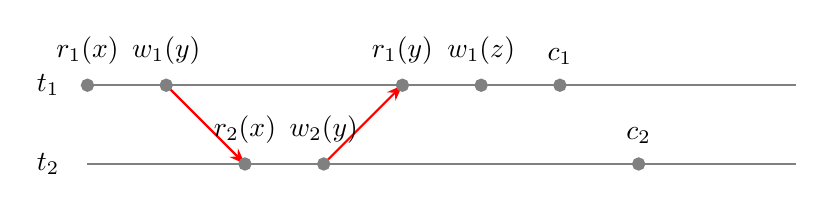
\begin{tikzpicture}[scale=1,transform shape,
>={Stealth[round]},thick,black!50,text=black,
every new ->/.style={shorten >=1pt},
graphs/every graph/.style={edges=rounded corners}]

  % \draw (0, 0) grid (10, 5);
  
  \draw (0.5, 2) node {$t_1$} (1, 2) -- (10, 2) node { };
  \draw (0.5, 1) node {$t_2$} (1, 1) -- (10, 1) node { };
 
  % $$ s = r_1(x) w_1(x) r_2(x) w_2(y) r_1(y) w_1(z) c_1 c_2 $$
  \coordinate (r1x) at (1,2);
  \coordinate (w1x) at (2,2);
  \coordinate (r2x) at (3,1);
  \coordinate (w2y) at (4,1);
  \coordinate (r1y) at (5,2);
  \coordinate (w1z) at (6,2);
  \coordinate (c1)  at (7,2);
  \coordinate (c2)  at (8,1);

  % conflict graph
  \draw [red,->,-{Stealth[length=2mm]}] (w1x) -- (r2x);
  \draw [red,->,-{Stealth[length=2mm]}] (w2y) -- (r1y);

  % step graph
  \filldraw (r1x) circle [radius=2pt] node [label=above:$r_1(x)$] {};
  \filldraw (w1x) circle [radius=2pt] node [label=above:$w_1(y)$] {};
  \filldraw (r2x) circle [radius=2pt] node [label=above:$r_2(x)$] {};
  \filldraw (w2y) circle [radius=2pt] node [label=above:$w_2(y)$] {};
  \filldraw (r1y) circle [radius=2pt] node [label=above:$r_1(y)$] {};
  \filldraw (w1z) circle [radius=2pt] node [label=above:$w_1(z)$] {};
  \filldraw (c1)  circle [radius=2pt] node [label=above:$c_1$] {};
  \filldraw (c2)  circle [radius=2pt] node [label=above:$c_2$] {};
\end{tikzpicture}
\end{document}
